\documentclass{beamer} % Класс презентации
% \documentclass[t]{beamer}  % выровнять текст на слайдах по верхнему краю
%  \documentclass[handout]{beamer} % Раздаточный материал
%\documentclass[aspectratio=169]{beamer} % Соотношение сторон

%\usetheme{Berkeley} % Тема оформления
%\usetheme{Bergen}
%\usetheme{Szeged}
\usetheme{Warsaw}
%\usetheme[numbers]{Statmod}

\usecolortheme{seahorse} %Цветовая схема
%\useinnertheme{circles}
%\useinnertheme{rectangles}

\usepackage{mathtext}          % русские буквы в формулах
\usepackage[T2A]{fontenc}            % внутренняя кодировка  TeX
\usepackage[utf8]{inputenc}         % кодировка исходного текста
%\usepackage{cmap}          % русский поиск в pdf
%\usepackage[english]% локализация и переносы
\usepackage{amsmath} % Математические окружения AMS
\usepackage{amsfonts} % Шрифты AMS
 \usepackage{amssymb} % Символы AMS
  \usepackage{mathtext} % Русские буквы в фомулах
  \usepackage{graphicx} % Вставить pdf- или png-файлы

  \usepackage{euscript} % Красивый шрифт
\setbeamercolor{item}{fg=blue!30}

  \usepackage{longtable}  % Длинные таблицы
  \usepackage{multirow} % Слияние строк в таблице

 \usepackage{indentfirst} % Отступ в первом абзаце.

 \newcommand*{\hm}[1]{#1\nobreak\discretionary{}%
            {\hbox{$\mathsurround=0pt #1$}}{}}
\newcommand{\argmin}{\operatornamewithlimits{argmin}}
 \usepackage{verbatim}

\usepackage{graphicx}  % Для вставки рисунков
\usepackage[update,prepend]{epstopdf} % EPS-рисунки конвертируются в PDF
\usepackage{wrapfig} % Обтекание рисунков текстом
\usepackage{booktabs}
\usepackage{changepage}


\usepackage{hyperref} % Гиперссылки



 \usepackage{etoolbox} % логические операторы

%строки ниже для вставления нумерации слайдов

\defbeamertemplate*{footline}{Warsaw} {%
\leavevmode%
\hbox{%
\begin{beamercolorbox}[wd=.5\paperwidth,ht=2.5ex,dp=1.125ex,leftskip=.3cm,rightskip=.3cm]{author in head/foot}%
\insertframenumber{}%
\hfill\insertshortauthor
\end{beamercolorbox}%
\begin{beamercolorbox}[wd=.5\paperwidth,ht=2.5ex,dp=1.125ex,leftskip=.3cm,rightskip=.3cm]{title in head/foot}%
\usebeamerfont{title in head/foot}\insertshorttitle
\end{beamercolorbox}
}%
\vskip0pt%
}
\usepackage[backend=biber, style=bwl-FU, citestyle=bwl-FU]{biblatex}
\addbibresource{bibliobase2.bib}

\DeclareMathOperator{\etr}{etr}
\DeclareMathOperator{\tr}{tr}
\DeclareMathOperator*{\argmax}{arg\,max}
%\DeclareMathOperator*{\argmin}{arg\,min}
\DeclareMathOperator{\E}{\mathbb{E}}
\DeclareMathOperator{\diag}{diag}
\DeclareMathOperator{\Var}{\mathbb{V}\mathrm{ar}}
\DeclareMathOperator{\chol}{chol}
\newcommand{\cN}{\mathcal{N}}
\newcommand{\cIW}{\mathcal{IW}}
\newcommand{\lag}{\EuScript{L}}

\newcommand{\prior}{\underline}
\newcommand{\post}{\overline}

\let\vec\relax
\DeclareMathOperator{\vec}{vec}




\author{Boris Demeshev\inst{1} \and Oxana Malakhovskaya\inst{2}}
\title[Forecasting with BVAR]{Forecasting Russian Macroeconomic Indicators with BVAR}

%\subtitle{Наша первая презентация}
%\date[Дата]{\today} % Если  \today, то можно просто не писать
\institute[National Research University Higher School of Economics]
{
  \inst{1}%
  Department of Applied Economics\\
  National Research University Higher School of Economics
  \and
  \inst{2}%
  Department of Theoretical Economics\\
  National Research University Higher School of Economics}

\date{36th International Symposium on Forecasting,  Santander, Spain, June 21, 2016}

\begin{document} % Конец преамбулы, начало текста.
\begin{frame} %{1}

\titlepage

\end{frame}



\begin{frame}{Motivation} %{2}
\begin{itemize}
%\item Accurate macroeconomic forecasts are  important for policy making.
%\item Central banks monitor a large set of macroeconomic indicators to determine the policy
%\end{itemize}
\item Accurate macroeconomic forecasts are extremely important for policy making.\\
\item Central banks monitor a large set of macroeconomic indicators to determine the policy.\\
\item Therefore, a model being used for forecasting purposes must be suitable for samples with large cross-sectional dimension to avoid a potential loss of relevant information.  
\end{itemize}
\end{frame}

%\begin{comment}

\begin{frame}{Motivation(2)}%{3}
\begin{itemize}
\item Vector autoregressions have become a  widely-used tool for forecasting. However,  unrestricted VARs bear the risk of overparameterization even for samples of moderate size.
\item Using of Bayesian estimation may alleviate this problem. The Bayesian shrinkage is done by imposing restrictions on parameters in the form of prior distributions. 
\item Recently many papers have claimed that, in terms of forecasting accuracy, medium and large BVAR outperform their small dimensional counterparts. 
\item Application of Bayesian econometrics on Russian data is scarce 
\end{itemize}
\end{frame}



\begin{frame}{Objective of the paper}%{4}
The objectives of the paper are:
\begin{itemize}
\item forecasting of macroeconomic indicators for Russian economy with BVARs of different sizes
\item comparing their forecasting accuracy with forecasting accuracy of competing  models (RW and unrestricted VARs)
\end{itemize}

Our underlying hypotheses are:
\begin{itemize}
\item BVARs outperform the competing models in terms of forecasting accuracy
\item high-dimensional BVARs forecast better than  low-dimensional ones 
\end{itemize}
\end{frame}

%\begin{frame}{BVAR на выборках большой размерности}%12
%\begin{itemize}
%\item Применение BVAR к выборкам большой размерности  было крайне ограничено до недавнего времени. Основная причина состояла в распространенной точке зрения, что байесовская регуляризация недостаточна для решения проблемы избыточной параметризации в выборках большой размерности.   
%\item \textit{\cite{demol_al_2008}} показали, что байесовские методы могут успешно применяться и выборках большой размерности, если жесткость регуляризации устанавливается в зависимости от размера выборки.
%\item \textit{\cite{banbura_al_2010}} подтвердили и развивли это утверждение с помощью  BVAR, постороенной на выборке американских временных рядов большой размерности.  
%\end{itemize}
%\end{frame}

\begin{frame}{BVAR in data-rich environment}%12
\begin{itemize}
\item While BVAR in low-dimensional space were widely used for macroeconomic analysis, their use for data-rich environment was limited until 2010. The reason was a general agreement that the Bayesian shrinkage is insufficient to solve the overparameterization problem in high cross-sectional dimension samples.
\item \cite{demol_al_2008} show that  the Bayesian methods can be successfully applied in data-rich environment if the degree of shrinkage is set relative to the cross-sectional dimension of the sample.
\item \cite{banbura_al_2010} confirm and develop this claim for BVAR applied to a large set of US time-series.
\end{itemize}
\end{frame}
  
\begin{frame}{VAR model}%{5}
Our baseline specification is a standard BVAR with a conjugate Normal-inverted Wishart prior.\\
\vspace{5mm}
VAR in reduced form: 
\begin{equation}
y_t =\Phi_{ex}+ \Phi_1 y_{t-1} + \Phi_2 y_{t-2} +\ldots + \Phi_p y_{t-p} + \varepsilon_t,\quad \varepsilon_t\sim N(0,\Sigma), 
\end{equation}
where $y_{it}$ is  a  $m\times 1$ vector of variables.\\
\vspace{8mm}
The model can also be written in a more compact way: 
\begin{equation}
Y=X\Phi+E,\label{var}
\end{equation}

where $Y=[y_1, y_2,\ldots, y_T]'$,$X=[x_1, x_2,\ldots, x_T]'$, $x_t=[ y'_{t-1} \ldots  y'_{t-p} \; 1]'$,  $\Phi=[\Phi_1 \ldots \Phi_p \; \Phi_{ex}]'$, $E=[\varepsilon_1, \varepsilon_2,\ldots, \varepsilon_T]'$ 

\end{frame}%{6}

\begin{frame}{Prior distribution}%{7}

The conjugate normal -- inverted Wishart prior is defined as:
\begin{equation}
\begin{cases} 
\Sigma\sim \cIW(\prior S, \prior \nu) \\
\Phi | \Sigma \sim \cN (\prior\Phi, \Sigma \otimes \prior\Omega)
\end{cases},
\end{equation}
%where $\prior \phi = \vec{ \prior \Phi}$ and: 

In addition to otherwise standard normal - inverse Wishart distribution we use two modifications of the prior that appeared to increase the forecasting performance in some other papers:
\begin{itemize}
\item sum-of-coefficients prior 
\item initial observation prior 
\end{itemize}
The overall tightness parameter is chosen endogenously depending on the sample dimension following \cite{banbura_al_2010}.
\end{frame}



%\begin{frame}{Bayesian estimation}
%Bayesian estimate combines a likelyhood function $L(Y|\Phi, \Sigma)$, with a prior distribution $p(\Phi, \Sigma|Y)$ and results in a posterior distributions of parameters $p(\Phi, \Sigma|Y)$. To find the distribution, a corollary from Bayes' rule is employed:
%
%\begin{equation}
%p(\Phi, \Sigma|Y)\propto p(\Phi,\Sigma) L(Y|\Phi,\Sigma)
%\end{equation}
%
%\end{frame}
%
%\begin{frame}{Conjugate Normal-inverted Wishart prior(1)}%{7}
%
%A  normal-inverted Wishart prior distribution can be written as: 
%\begin{equation}
%\begin{cases} 
%\Sigma\sim \cIW(\prior S, \prior \nu) \\
%\Phi | \Sigma \sim \cN (\prior\Phi, \Sigma \otimes \prior\Omega)
%\end{cases},
%\end{equation}
%%where $\prior \phi = \vec{ \prior \Phi}$ and: 
%
% where $\prior\Phi=[\prior\Phi_1 \ldots \prior\Phi_p \; \prior\Phi_{ex}]'$ and 
%
%
%\begin{equation}
%(\prior\Phi_l)_{ij}=
%\begin{cases}
%\delta_i\; i=j, l=1;\\
%0,\;\text{ otherwise }
%\end{cases} 
%\end{equation}
%\end{frame}
%
%\begin{frame}{Conjugate Normal-inverted Wishart prior(2)}%{8}
%\begin{equation}
%\prior \Omega=\begin{pmatrix} \label{prior_omega1}
%\prior \Omega_{lag=1}&0_{m\times m}&\cdots&0_{m\times m}&0_{m\times 1}\\
%0_{m\times m}& \prior\Omega_{lag=2}& \cdots &0_{m\times m}&0_{m\times 1}\\
%\vdots &\vdots& \ddots&\vdots& \vdots\\
%0_{m\times m}&0_{m\times m}&\cdots&\prior\Omega_{lag=p} & 0_{m\times 1}\\
%0_{1\times m}&0_{1\times m}&\cdots&0_{1\times m}&\prior \Omega_{const}
%\end{pmatrix} 
%\end{equation}
%
%$\prior \Omega_{lag=l}$ is $m\times m$ matrix, and its diagonal elements are: 
%\begin{equation}
%(\prior \Omega_{lag=l})_{jj} \label{prior_omega2}
%=\left(\frac{\lambda_{tight}}{l^{\lambda_{lag}}\hat\sigma_j}\right)^2
%\quad
%\prior \Omega_{const}=\lambda_{const}^2 
%\end{equation}
%Matrix $S$ is also diagonal with elements defined as:
%\begin{equation}
%(\prior S)_{ii}= (\prior \nu- m- 1) \hat\sigma^2_{i}
%\end{equation}
%
%Degrees of freedom parameter is chosen to be:
%\begin{equation}
%\prior \nu \geq\max\lbrace m+2, m+2h-T\rbrace
%\end{equation}
%\end{frame}
%
%\begin{frame}{ Modifications of Conjugate N-IW prior}%{9}
%\begin{itemize}
%\item The literature has suggested that forecasting performance can be improved if the conjugate N-IW distribution is complemented with sum-of-coefficients  and dummy initial observation priors  proposed by \cite{doan_al_1984} and \cite{sims_1993}, respectively.  
%\item Sum-of-coefficients prior constrains the sum of coefficients and may be interpreted as <<inexact differencing>>. It introduces the following  hyperparameters: $\lambda_{sc}$ and $\mu_i$, $i=1,\ldots,m$
%\item Dummy initial observation prior expresses a belief that variables can have a common stochastic trend and introduces     only one hyperparameter $\lambda_{io}$ 
%\end{itemize}
%\end{frame}
%
%
%
%\begin{frame}{Hyperparameters choice(1)}%10
%\begin{gather}
% \prior\Phi = \prior\Phi (\delta)\\
% \prior \Omega=\prior \Omega (\lambda_{tight},\lambda_{lag}, \lambda_{const}, \hat \sigma)\\
% \prior S=\prior S (\hat \sigma)
%\end{gather}
%
%In literature on BVAR  vector $\delta$ is defined in several ways:
%\begin{itemize}
%\item all $\delta_i=1$ (as in original Minnesota prior)
%\item $\delta_i=0$ for stationary series and $\delta_i=1$ for nonstationary series
%\item $\delta_i<1$ for stationary series and $\delta_i=1$ for nonstationary series 
%\item $\delta_i$ to be equal to first-lag OLS estimate in AR(p) model etc.
%\end{itemize}
% $\hat\sigma_i$ is usually chosen to be equal to standard deviation of residuals in AR(1) or AR(p) model  for variable $i$. \\
%\end{frame}
%
%\begin{frame}{Hyperparameters choice(2)}%11
%\begin{gather}
% \prior\Phi = \prior\Phi (\delta)\\
% \prior \Omega=\prior \Omega (\lambda_{tight},\lambda_{lag}, \lambda_{const}, \hat \sigma)\\
% \prior S=\prior S (\hat \sigma)
%\end{gather}
% We fix $\lambda_{lag}$ at unity (as in majority of other studies) and $\lambda_{const}=Inf$ and we optimize on $\lambda_{tight}$. 
%We follow \cite{sims_zha_1998} and choose $\mu=\frac{1}{p}\sum_{t=1}^p y_t$. According to common practice we set $\lambda_{sc}=10\lambda_{tight}$ and $\lambda_{io}=1$, $\prior \nu$ is equal to $m+2$. 
%\end{frame}


%\begin{frame}{Algorithms for choosing $\lambda_{tight}$}%13
%Two ways of choosing optimal $\lambda_{tight}$ in the literature are: 
%\begin{enumerate}
%\item The shrinkage must be so tight to avoid an overparameterization. Three-variable unrestricted VAR is assumed to be parsimonious enough and it does not need any shrinkage. So $\lambda_{tight}$ is chosen in such a way that average in-sample  BVAR forecast on a training sample for several variables of interest is the same as 3-variable unrestricted VAR. This method was introduced by \cite{banbura_al_2010}
%\item $\lambda_{tight}$ is chosen so that to maximize the marginal data density. The algorithm  was introduced by \cite{doan_al_1984} and used recently by \cite{carriero_al_2015}   
%\end{enumerate}
%
%\end{frame}

\begin{frame}{Our dataset}%14
\begin{itemize}
\item 23 monthly time series running from January 1996 to April 2015 
\item Series demonstrating seasonal fluctuations are seasonally adjusted 
\item Logarithms are applied to most of the series, with the exception of those already expressed in rates.
\end{itemize}
\end{frame}


\begin{frame}{Estimated models} %15
VAR in compact  form:

\begin{equation}
Y=X\Phi+E,\label{var}
\end{equation}
\begin{center}
\begin{tabular}{p{2.5cm}l}
\toprule
VAR3/BVAR3&$Y=\lbrace IP, CPI, R \rbrace$\\
VAR4/BVAR4 &$Y=\lbrace IP, CPI, R, Z\rbrace$ \\
VAR6/BVAR6& $Y=\lbrace IP, CPI, R, M2, REER, OPI \rbrace$ \\
VAR7/BVAR7&$Y=\lbrace IP, CPI, R, M2, REER, OPI, W \rbrace$\\
BVAR23&$Y$ includes all 23 variables from the dataset\\
\bottomrule
\end{tabular}
\end{center}
$IP$ - industrial product index, $CPI$ - consumer price index, $R$ - nominal interbank rate, $M2$ - monetary aggregate M2, $REER$ - real effective exchange rate, $OPI$ - Brent oil price index. $Z$ is any variable from the dataset besides $IP$, $CPI$ and $R$.  $W$ is any variable from the dataset besides $IP$, $CPI$, $R$, $M2$,$REER$, and $OPI$.
\end{frame}

\begin{frame}{Estimation scheme}%16
%\begin{center}
 \hspace*{-0.9cm}
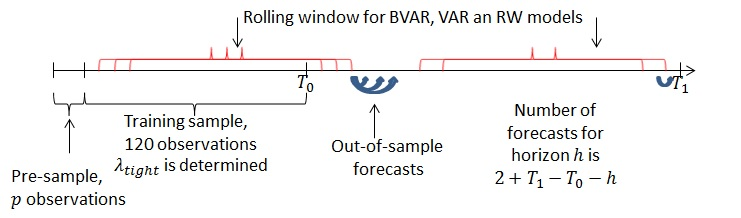
\includegraphics[scale=0.65]{estimation_scheme2.jpg}
%\end{center}
\end{frame}

\begin{frame}{Results(1)}%16
\vspace{-5mm}
\begin{center}
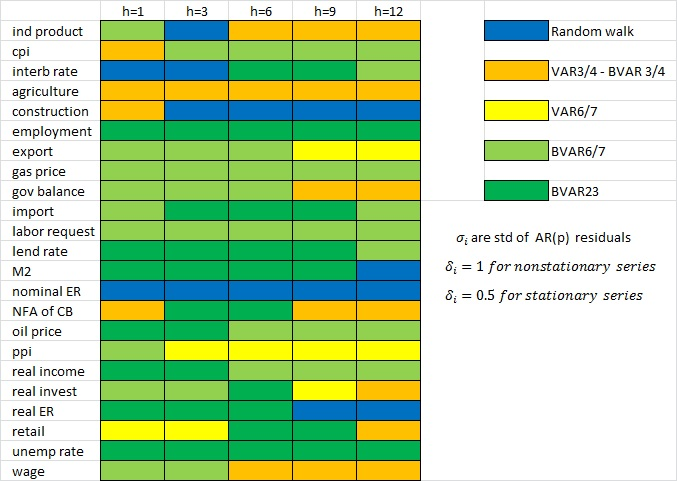
\includegraphics[scale=0.60]{hyper1.jpg}
\end{center}
\end{frame}

\begin{frame}{Results(2)} %17
\vspace{-5mm}
\begin{center}
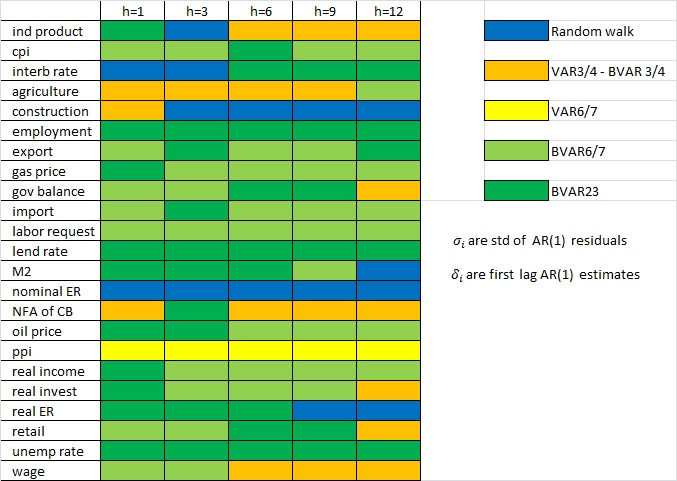
\includegraphics[scale=0.60]{hyper2.jpg}
\end{center}
\end{frame}

\begin{frame}{Forecast accuracy}
We measure out-of-sample forecast accuracy in terms of mean squared forecast error... 
\begin{equation}
MSFE_{var,h}^{\lambda,m}=\frac{1}{T_1-T_0-h+1}\sum_{\tau=T_0}^{T_1-h} (y_{var,\tau+h|\tau}^{\lambda,m}-y_{var,\tau+h|\tau})^2
\end{equation}

... and report relative MSFE, i.e. the ratio of MSFE of the model in question by the MSFE of a benchmark (RW with drift in our case): 

\begin{equation}
RMSFE=\frac{MSFE_{var,h}^{\lambda,m}}{MSFE_{var,h}^0}
\end{equation}
where $var$ is any variable in the dataset
\end{frame}


\begin{frame}{Relative MSFE(1)} %18
\vspace{-5mm}
\begin{center}
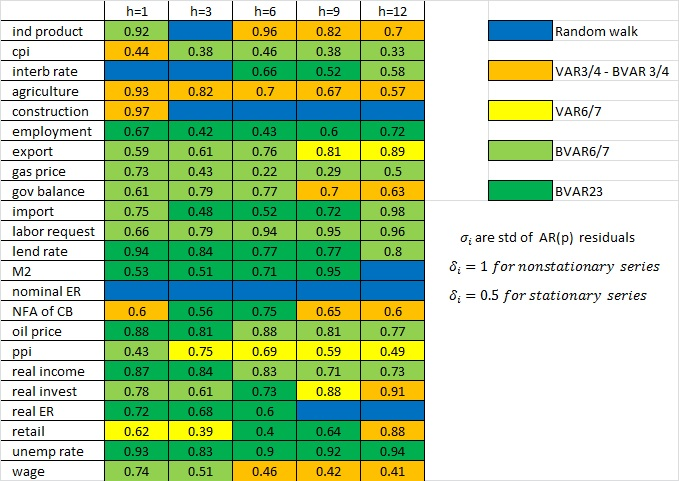
\includegraphics[scale=0.60]{hyper3.jpg}
\end{center}
\end{frame}

\begin{frame}{Relative MSFE(2)} %19
\vspace{-5mm}
\begin{center}
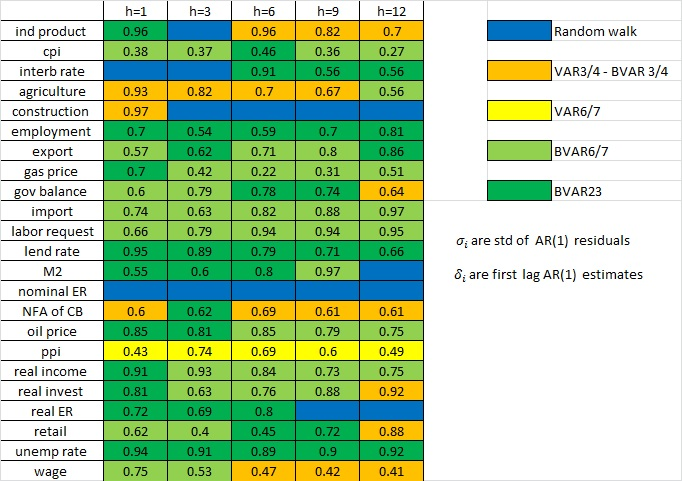
\includegraphics[scale=0.60]{hyper4.jpg}
\end{center}
\end{frame}

\begin{frame}{Robustness check}
\begin{adjustwidth}{-1.5em}{-1.5em}
\vspace{-5mm}
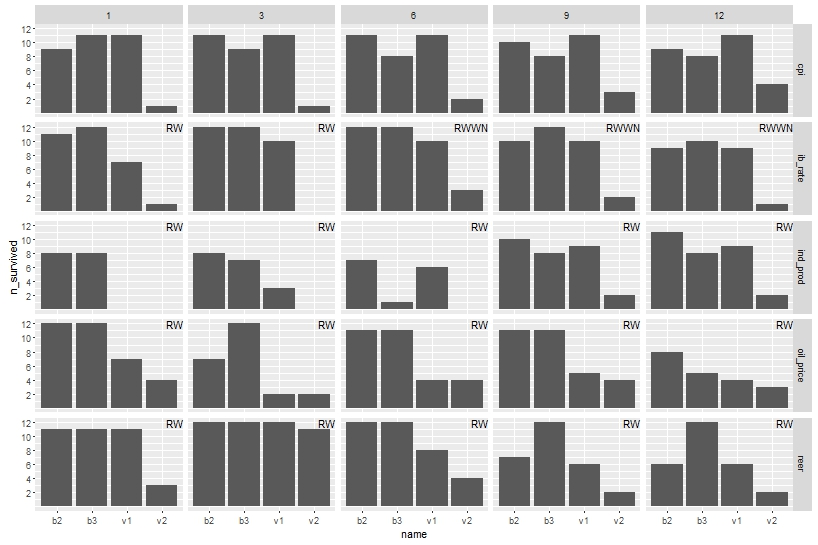
\includegraphics[scale=0.42]{model_selection.jpeg}
\end{adjustwidth}
\end{frame}




\begin{frame}{Interpretation of the results} %20
\begin{itemize}
\item For many variables and forecasting horizons in interest, BVAR outperforms random walk and unrestricted VAR.
\item Though medium BVAR is the best option for some cases, it is often beaten by a BVAR model with relatively low number of variables (6 or 7). 
\item For some variables and some forecasting horizons VARs (either restricted or not) cannot beat RW, for example, nominal exchange rate (long-lasting consensus in economics)
\item Nonetheless, the oil price index can be forecast by BVAR much better than by RW.
\end{itemize}
\end{frame}

\begin{frame}{Conclusion}%21
\begin{itemize}
\item In the paper, we estimate BVAR models of different size and compare their forecasting performance with RW with drift and unrestricted VAR models for 23 variables and 5 different forecast horizons. 
\item We show that for a majority of variables of interest BVAR produces better forecasting results than the competing models. 
\item However, we cannot confirm a conclusion of some studies that high-dimensional BVARs forecast better than low-dimensional models. For many variables in our sample and forecasting horizons a 6- or 7-variable BVAR can beat a 23-variable BVAR in terms of forecasting accuracy.
\end{itemize}
\end{frame}

\begin{frame}%22
\begin{center}
THANK YOU FOR YOUR ATTENTION!
\vspace{1cm}
\end{center}
Boris Demeshev: boris.demeshev@gmail.com\\
Oxana Malakhovskaya: omalakhovskaya@hse.ru\\
Link to the repository: https://github.com/bdemeshev/bvar\_om
\end{frame}
\end{document}

